%\documentclass[unicode]{beamer}
\documentclass[unicode,hyperref={unicode=true}]{beamer}
\mode<presentation>
{
%  \useoutertheme{shadow}
%  \useinnertheme{rounded}
  \usecolortheme[RGB={55,109,160}]{structure}
%  \usetheme[height=7mm]{Rochester}
%  \usetheme{default}
%  \usetheme{Warsaw}
%  \usetheme{Frankfurt}
  \usetheme{Dresden}
%  \setbeamercolor{normal text}{bg=black,fg=white}
  \setbeamertemplate{navigation symbols}{}
  \setbeamertemplate{blocks}[rounded][shadow=true]
  \setbeamertemplate{items}[ball]
  \setbeamercovered{invisible}
}

\defbeamertemplate*{footline}{infolines theme}
{
  \leavevmode%
  \hbox{%
  \begin{beamercolorbox}[wd=\paperwidth,ht=2.25ex,dp=1ex,right]{date in head/foot}%
    \insertframenumber{} / \inserttotalframenumber\hspace*{2ex}
  \end{beamercolorbox}}%
  \vskip0pt%
}

% \setbeamertemplate{headline}{
%   \leavevmode
%  \hbox{%
%  \begin{beamercolorbox}[wd=\paperwidth,ht=3.25ex,dp=1ex,right]{date in head/foot}%
%    Институт системного программирования \\ Российская академия наук
%    \insertframenumber{} / \inserttotalframenumber\hspace*{2ex}
%  \end{beamercolorbox}}%
%  \vskip0pt%
%   \includegraphics[width=\textwidth]{logo-cmb.png}%
%}

\setbeamertemplate{headline}{
	\begin{beamercolorbox}[wd=\paperwidth,ht=3.25ex,dp=1ex,left]{date in head/foot}
		~~\insertsection
	\end{beamercolorbox}
}

\setbeamerfont{section title}{parent=title}
\setbeamercolor{section title}{parent=titlelike}
\defbeamertemplate*{section page kb}{default}[1][]
{
  \centering
	\begin{beamercolorbox}[sep=8pt,center,#1]{section title}
	  \usebeamerfont{section title}\insertsection\par
	\end{beamercolorbox}
}
\newcommand*{\sectionpagekb}{\usebeamertemplate*{section page kb}}
\setbeamercolor{block title}{use=structure,fg=white,bg=structure.fg!75!black}

\usepackage{etex}
\usepackage[T1]{fontenc}
\usepackage[utf8]{inputenc}
\usepackage[russian]{babel}
\usepackage{graphicx}
\usepackage{fancyvrb}
\usepackage{shortvrb}
\usepackage{amsthm}
\usepackage[]{url}
%\MakeShortVerb{!}
\usepackage{listings}
\lstset{ %
    stringstyle=\color{red},
    extendedchars=\true,
    inputencoding=utf8,
    columns=fixed,keepspaces
}
\usepackage{enumerate}
\usepackage{tikz}
\usepackage{xy}
\usepackage{algorithm}
\usepackage{algorithmicx}
\usepackage{algpseudocode}
\usepackage{latexsym}
\usepackage{subfig}
\usepackage{tikz}
\usepackage{dirtree}
\usetikzlibrary{positioning,arrows}
%\lstset{basicstyle=\ttfamily,language=lisp}

\theoremstyle{definition}
\newtheorem{mydef}{Определение}
\theoremstyle{plain}
\newtheorem{stmt}{Утверждение}
%\theoremstyle{plain}
%\newtheorem{lemma}{Лемма}

\title[]
{Автоматизация разработки моделей устройств и вычислительных машин для QEMU}

\author[]{Ефимов Василий}

\institute[]{ИСП РАН}

\date[]{18 октября 2017}

\begin{document}

\begin{frame}
\titlepage
\end{frame}



\begin{frame}{Проблема}
\begin{itemize}
\item Чтобы задействовать все возможности динамического анализа нужен эмулятор с
поддержкой соответствующей вычислительной машины.
В данном случае используется эмулятор QEMU.
\vfill
\item Разработка моделей устройств и машин для QEMU~--- это трудоёмкий процесс.
В связи с повысившейся заинтересованностью в расширении QEMU новыми
машинами, требуется его ускорить.
\vfill
\item Ускорения предлагается достичь за счёт автоматизации.
\end{itemize}
\end{frame}



\begin{frame}{Цели работы}
Целью работы является автоматизация процесса разработки моделей устройств и
вычислительных машин для эмулятора QEMU.

\vfill

{Для достижения поставленной цели были выполнены следующие задачи:}

\begin{itemize}
\item анализ QEMU и поиск в исследуемом процессе автоматизируемых этапов;
\item разработка и реализация метода автоматизации;
\item повышение удобства использования реализованного инструмента.
\end{itemize}
\end{frame}



\section{Подход к автоматизации}
\begin{frame}
\sectionpagekb
\begin{itemize}
\item Процесс до автоматизации и его особенности
\item Объектная модель QEMU (QOM)
\item Особенности API QEMU для моделирования устройств и компоновки виртуальных
машин (VM)
\item Предлагаемый автоматизированный процесс
\item Похожие результаты
\end{itemize}
\end{frame}



\begin{frame}{Процесс разработки до автоматизации}
\begin{center}
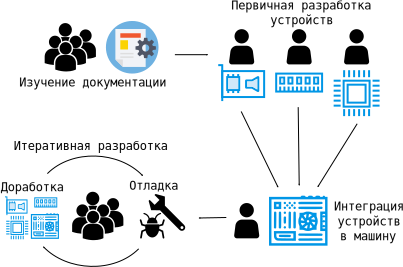
\includegraphics[height=0.8\textheight]{workflow-old.png}
\end{center}
\end{frame}



\begin{frame}{Основные сложности}
\begin{itemize}
\item Пока нет большинства устройств, скомпоновать машину нельзя.
\item Устройство <<в вакууме>> ограничено в отладке. Чтобы отлаживать
устройство необходимо внедрить его в машину и запустить в ней ПО.
\item Модели содержат много однотипного формального кода, который приходится
писать, копировать и править для каждой модели.
\end{itemize}
\end{frame}



\begin{frame}{Объектная модель QEMU (QOM)}
\begin{minipage}{0.49\textwidth}
\dirtree{%
.1 object .
    .2 machine .
    .2 device .
        .3 sys-bus-device .
            .4 модельный ряд .
               .5 конкретное\\устройство .
        .3 pci-device .
        .3 cpu, {...} .
    .2 bus .
        .3 PCI .
            .4 PCIE .
        .3 System .
        .3 usb-bus, {...}.
    .2 irq .
    .2 qemu:memory-region .
}
\hfill
\end{minipage}
\hfill
\begin{minipage}{0.49\textwidth}
\begin{itemize}
\item ООП на Си (похоже на gobject из Gnome library)
\item Базовое понятие ---~тип~(type)
\item тип =~\textit{класс}~(class) +~\textit{экземпляр}~(instance)
\item класс/экземпляр =~\textit{структура}~(\texttt{struct}, Си)
+~\textit{конструктор}~(функция обратного вызова, Си)
\item \texttt{object} ---~один из типов, добавляющий
\textit{свойства}~(property) к классу и экземпляру
\end{itemize}
\end{minipage}
\end{frame}



\begin{frame}{API QEMU для моделирования устройства}
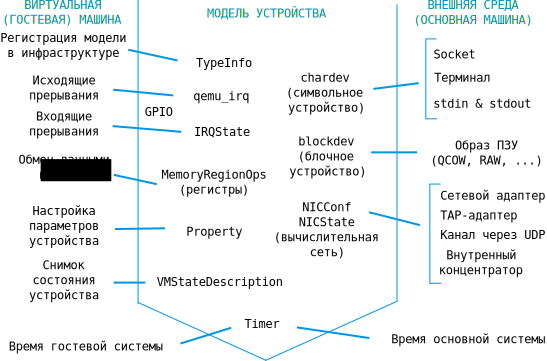
\includegraphics[width=\linewidth]{device-model-ex.png}
\vfill
\it{*Стрелками показано распространение данных.}
\end{frame}



\begin{frame}{Особенности разработки устройства}

\begin{minipage}{0.6\textwidth}

\includegraphics[width=\linewidth]{device-model.png}
\end{minipage}
\begin{minipage}{0.38\textwidth}
\begin{itemize}
\item Развитый обобщающий API
\item Много формального интерфейсного кода
\item Индивидуальный код сосредоточен в чётко определённых местах
\end{itemize}
\end{minipage}

\begin{center}
Можно по краткому перечню параметров сгенерировать сравнительно большую
заготовку.
\end{center}

\end{frame}


\begin{frame}[fragile]{Типовой способ компоновки VM}
\lstset{language=C}
\begin{lstlisting}
/* Создание экземпляра устройства. */
dev = qdev_create(parent_bus, QOM_TYPE_NAME);
/* Задание свойств. */
object_property_set_TYPE(dev,
                         PROP_VALUE, PROP_NAME,
                         ...);
/* " Реализация" экземпляра устройства. */
qdev_init_nofail(dev);
/* Отображение регистров. */
sysbus_mmio_map(dev, REG_INDEX, REG_ADDRESS);
/* Связывание прерываний. */
my_incoming_irq = qdev_get_gpio_in(dev,
                                   IN_IRQ_INDEX);
sysbus_connect_irq(dev, OUT_IRQ_INDEX,
                   neighbour_incoming_irq);
\end{lstlisting}
\end{frame}


\begin{frame}{Особенности компоновки VM}

\begin{itemize}
\item Декларативный характер определения
\item Применяется объектная модель
\item Сложная система взаимосвязей, тяжело поддающаяся восприятию в форме
программного кода
\end{itemize}

\begin{center}
Требуется отобразить VM на схеме в графическом редакторе.
Редактор должен генерировать заготовку модели машины.
\end{center}

\end{frame}



\begin{frame}{Предлагаемый процесс разработки}
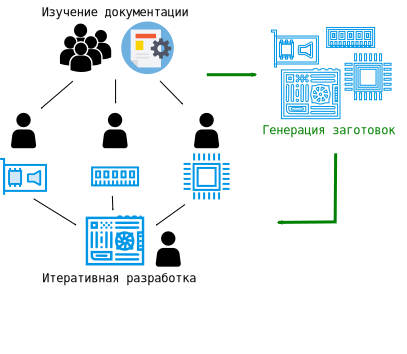
\includegraphics[width=\linewidth]{workflow.png}
\end{frame}



\begin{frame}[fragile]{Похожие результаты}
\begin{center}
\begin{tabular}{l|ccc}
Эмулятор/  & \multicolumn{2}{c}{Прототипирование} & Автоматизация            \\
Симулятор  & GUI & API                            &                          \\
\hline
Simics     &  +  & C++, Python                    & DML \(\rightarrow\) C++  \\
AMD SimNow &  +  & C++                            & -                        \\
gem5       &  -  & C++, Python                    & -                        \\
OVPSim     &  -  & C                              & TCL \(\rightarrow\) C    \\
QEMU       &  -  & C                              & -                        \\
\end{tabular}
\end{center}
\end{frame}



\section{Разработанный инструмент}
\begin{frame}{}
\sectionpagekb
\begin{itemize}
\item Архитектура
\item Формат хранения настроек генерации
\item Задание параметров генерации заготовок устройств и машин
\item Графический интерфейс пользователя (ГИП)
\item Особенности генерации кода
\item Вспомогательные модели генератора кода
\item Взаимосвязь с существующим кодом QEMU
\end{itemize}
\end{frame}{}


\begin{frame}{}
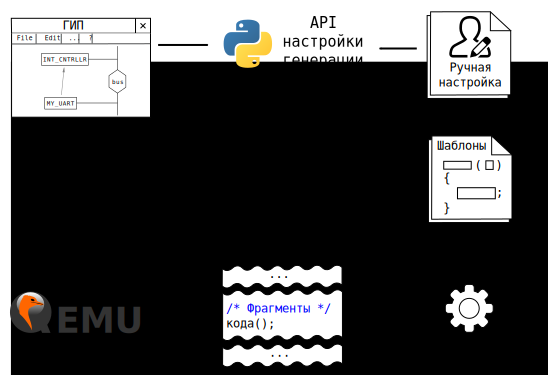
\includegraphics[width=\linewidth]{main.png}
\end{frame}



\begin{frame}{Формат хранения настроек генерации заготовок}
Настройки хранятся в форме кода на Python.
\vfill
\dirtree{%
.1 object .
    .2 QProject .
        .3 GUIProject .
    .2 QOMDescription .
        .3 SysBusDeviceDescription .
        .3 PCIExpressDeviceDescription .
        .3 MachineNode .
}
\vfill
\texttt{object} --- базовый класс языка Python.\\
\texttt{QProject} --- контейнер с описаниями заготовок.\\
\texttt{GUIProject} --- дополнительные настройки для ГИП.\\
\texttt{QOMDescription} --- базовый класс для хранения настроек генерации
конкретной заготовки.\\
\texttt{MachineNode} --- контейнер для описания состава машины.
\end{frame}




\begin{frame}{Возможности настройки генерации устройства}
\begin{center}
\begin{tabular}{l|r}
Класс устройства & Настройки \\
\hline
Любой            & таймеры \\
                 & символьные и блочные устройства \\
                 & сетевой интерфейс \\
\hline
Устройство       & MMIO \\
системной        & PMIO \\
шины             & in/out IRQ \\
\hline
Функция          & BAR \\
PCI(E)           & out IRQ (INTx) \\
устройства       & MSI(X) \\
                 & идентификационная информация
\end{tabular}
\end{center}
\end{frame}



\begin{frame}[fragile]{Пример кода настройки генерации устройства}
\begin{center}
Собирательное устройство <<CISCO Remote>> из С2600
\end{center}
\lstset{language=Python}
\begin{lstlisting}
obj43 = SysBusDeviceDescription(
    name = "CISCO Remote", # имя модели
    directory = "char",    # папка модели
# Параметры генерации заготовок API QEMU
#    out_irq_num = 0,      - значения по умолчанию
#    in_irq_num = 0,         явно указывать не нужно
    mmio_num = 0x1,
#    pio_num = 0,
#    nic_num = 0,
#    timer_num = 0,
    char_num = 0x1,
    block_num = 0x1
)
\end{lstlisting}
\end{frame}

\begin{frame}{Пример настройки генерации устройства в ГИП}
\begin{center}
PCI Fast Ethernet контроллер из С2600
\end{center}
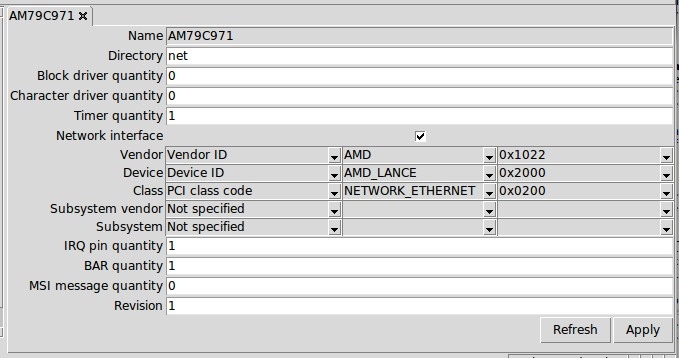
\includegraphics[width=\linewidth]{AM79C971.jpg}
\end{frame}



\begin{frame}[fragile]{Описание состава виртуальной машины}

\begin{minipage}{0.61\textwidth}
\dirtree{%
.1 Node .
    .2 BusNode .
        .3 SystemBusNode .
        .3 PCIExpressBusNode .
        .3 [ISA, IDE, I2C]BusNode .
    .2 DeviceNode .
        .3 SystemBusDeviceNode .
        .3 PCIExpressDeviceNode .
    .2 IRQLine .
    .2 IRQHub .
    .2 MemoryNode .
        .3 MemoryLeafNode .
            .4 MemoryAliasNode .
            .4 MemoryRAMNode .
            .4 MemoryROMNode .
}
\end{minipage}
\begin{minipage}{0.37\textwidth}
Иерархия основана на API QEMU.\\
 \\
Шины и устройства наследуются по принадлежности к стандарту шины.\\
 \\
\texttt{IRQHub} --- абстракция, позволяющая доставить одно прерывание к
нескольким устройствам.
\end{minipage}
\end{frame}



\begin{frame}[fragile]{Особенности API компоновки VM}
Параметры интеграции элементов задаются при создании объекта (обрабатываются
конструктором).\\
\lstset{language=Python}
\begin{lstlisting}
PCIExpressDeviceNode(
    qom_type,            # имя типа устройства (QOM)
    pci_express_bus,     # родительская шина
    slot, function,      # адрес на шине
    *a, **kw             # прочие параметры
)
\end{lstlisting}
\vfill
Ввиду возможности циклических связей между объектами, \textit{\textbf{после}}
создания объекта добавляются следующие параметры:
\begin{itemize}
\item \textit{для устройств}: свойства и связи с дочерними шинами;
\item \textit{для памяти}: вложенность участков.
\end{itemize}
\end{frame}



\begin{frame}{Общий вид схемы машины}
\begin{minipage}[b]{0.71\textwidth}
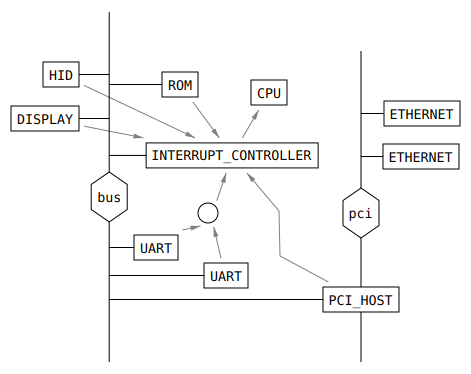
\includegraphics[width=\linewidth]{machine-example.png}\\
(упрощенная схема типового криптомаршрутизатора)
\end{minipage}
\hfill
\begin{minipage}[t]{0.24\textwidth}
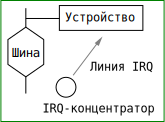
\includegraphics[width=\linewidth]{legend.png}\\
обозначения
\end{minipage}
\end{frame}



\begin{frame}[fragile]{Пример кода настройки интеграции устройства}
\lstset{language=Python}
\begin{lstlisting}
obj3 = SystemBusDeviceNode(
    qom_type = "TYPE_CISCO_REMOTE",
    system_bus = obj1,
    mmio = [ 0xf6000000 ]
)
obj3.properties.extend([
    QOMPropertyValue(QOMPropertyTypeString,
        "chardev", "serial2"),
    QOMPropertyValue(QOMPropertyTypeString,
        "eeprom_c2600_mb", "eeprom-c2600-mb"),
    QOMPropertyValue(QOMPropertyTypeLink,
        "nvram", obj2),
    QOMPropertyValue(QOMPropertyTypeInteger,
        "remote_cpu_type", 0x2)
])
\end{lstlisting}

\end{frame}



\begin{frame}{Пример настройки интеграции устройства в ГИП}
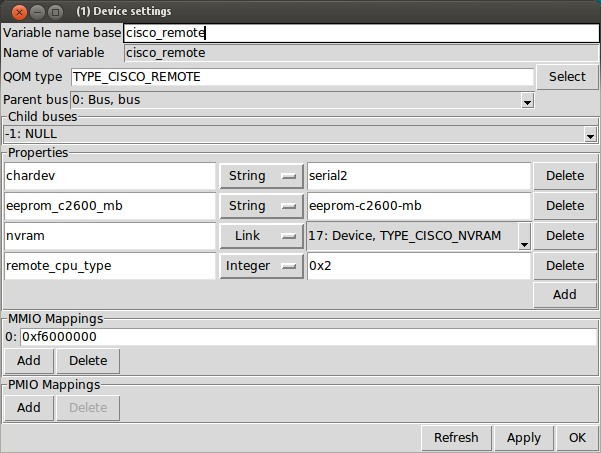
\includegraphics[height=0.9\textheight]{REMOTE.jpg}
\end{frame}



\begin{frame}[fragile]{Пример кода настройки интеграции шины}
\lstset{language=Python}
\begin{lstlisting}
obj18 = PCIExpressBusNode(
    host_bridge = obj13,
    var_base = "pci"
)
\end{lstlisting}
\vfill
\begin{itemize}
\item Нужно указать только мост (родительское устройство).
\item Устройства-дети привязываются при создании этих устройств.
\item Параметров генерации шины много, но все они задаются при наследовании:
\end{itemize}
\vfill
\lstset{language=Python}
\begin{lstlisting}
class BusNode(Node):
    def __init__(self, parent = None,
        c_type = "BusState", cast = "BUS",
        child_name = "bus", force_index = True,
        var_base = "bus", **kw
    ):
\end{lstlisting}
\end{frame}



\begin{frame}{Пример настройки интеграции шины в ГИП}
\begin{center}
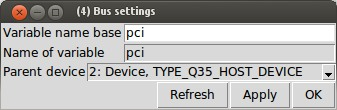
\includegraphics[width=0.7\linewidth]{bus_widget.jpg}
\end{center}
\end{frame}



\begin{frame}[fragile]{Пример кода настройки линии IRQ}
\lstset{language=Python}
\begin{lstlisting}
obj31 = IRQLine(
    src_dev = obj13,
    dst_dev = obj12,
    src_irq_idx = "3",
    dst_irq_idx = "3",
    dst_irq_name = "SYSBUS_DEVICE_GPIO_IRQ"
)
\end{lstlisting}
\vfill
\begin{itemize}
\item Точки подключения прерываний к устройству собраны в
\textit{\textbf{именованные}}
группы.
\item Внутри группы точки \textit{\textbf{нумеруются}}, начиная с \texttt{0}.
\item Если имя группы не указано, то подразумевается
\texttt{"unnamed-gpio-in"} / \texttt{"*-out"}.
\end{itemize}
\end{frame}



\begin{frame}{Пример настройки линии IRQ в ГИП}
\begin{center}
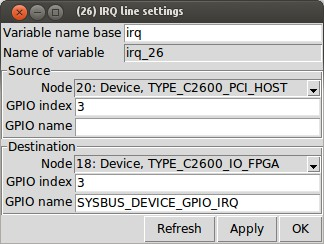
\includegraphics[height=0.8\textheight]{irq_widget.jpg}
\end{center}
\end{frame}



\begin{frame}[fragile]{Пример кода настройки интеграции памяти}
\lstset{language=Python}
\begin{lstlisting}
alias = MemoryAliasNode(
    name = "test_alias", # отладочное имя
    size = 0x1000,       # собственный размер

    alias_to = isa_bios, # cсылается на адрес 0x4000
    offset = 0x4000      # относительно начала
)                        # isa_bios

pci_as.add_child(        # включение alias в участок
    child = alias,       # pci_as со смещением
    offset = 0xdeadbeef, # 0xdeadbeef и низким
    priority = -1        # приоритетом
)
\end{lstlisting}
\end{frame}



\begin{frame}{Пример настройки интеграции памяти в ГИП}
\begin{center}
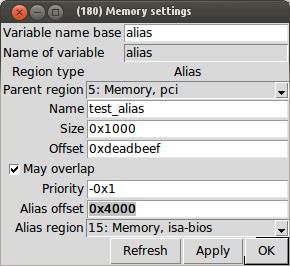
\includegraphics[height=0.7\textheight]{test_alias.jpg}
\end{center}
\end{frame}



\begin{frame}{Пример дерева памяти в ГИП}
\begin{center}
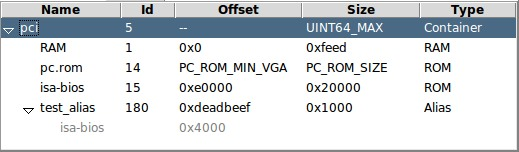
\includegraphics[width=\textwidth]{memory_tree.jpg}
\end{center}
\end{frame}



\begin{frame}{Требования к генерируемому коду:}
\begin{itemize}
\item синтаксическая корректность~--- возможность сразу после генерации
сосредоточиться на написании индивидуальной части кода;
\begin{itemize}
\item подключены все заголовки;
\item правильный порядок фрагментов кода;
\end{itemize}
\item соответствие стилю программирования~--- минимизация количества времени,
требуемого на последующий рефакторинг;
\begin{itemize}
\item соблюдены отступы и правила переноса;
\item соблюдены соглашения об именовании символов;
\item семантическая группировка фрагментов кода.
\end{itemize}
\end{itemize}
\end{frame}



\begin{frame}{Вспомогательные модели генератора}

\includegraphics[height=0.9\textheight]{generation.png}
\end{frame}



\begin{frame}{Модель гибридного языка}
\dirtree{%
.1 object .
    .2 Source\ \ \ \ \ \ \ \ \ \ \ \ \ - контейнер.
        .3 Header.
    .2 Type .
        .3 Structure\ \ \ \ \ \ \ - для Си.
        .3 Function .
        .3 Pointer .
        .3 Enumeration .
        .3 Macro\ \ \ \ \ \ \ \ \ \ \ - для препроцессора.
        .3 TypeReference\ \ \ - межфайловая связь.
    .2 Variable\ \ \ \ \ \ \ \ \ \ \ - Type + имя.
    .2 Initializer\ \ \ \ \ \ \ \ \ \ \ \ \{ + начальное значение \}.
    .2 Usage\ \ \ \ \ \ \ \ \ \ \ \ \ \ - Type/Variable + Initializer.
}

\vfill
Модель описывает содержимое файла с исходным кодом.
\end{frame}



\begin{frame}[fragile]{Тип}
\lstset{language=Python}
\begin{lstlisting}
Type(name, incomplete = True, base = False)
\end{lstlisting}
\vfill
\begin{itemize}
\item \texttt{name} --- уникальный строковый идентификатор; совпадает с
    именем соответствующего Си-типа, функции или макроса.
\item \texttt{incomplete} --- нельзя создать \textit{переменную} такого типа, но
    можно создать \textit{указатель} на такой тип или зависимость от него. Все
    классы-потомки являются завершёнными.
\item \texttt{base} --- тип не зависит от других типов: не требуется
    генерировать код, обеспечивающий его <<видимость>>.
\end{itemize}
\end{frame}



\begin{frame}[fragile]{Указатель}
\lstset{language=Python}
\begin{lstlisting}
Pointer(_type, name = None, const = False)
\end{lstlisting}
\vfill
\begin{itemize}
\item Описывает указатель на Си-тип или функцию (\texttt{\_type}).
\item \texttt{name} --- позволяет создать \textit{именованный} указатель,
    например:\\

\lstset{language=C}
\begin{lstlisting}
typedef const char * pstr_t;
typedef int (*my_callback_t) (char, void *);
\end{lstlisting}

    Имя именованного указателя --- это имя типа: оно должно быть уникально.
    Безымянные указатели такого ограничения не имеют и используются в
    конструкциях вида:

\lstset{language=C}
\begin{lstlisting}
const char *my_string;
int *p;
\end{lstlisting}


\item \texttt{const} --- создаёт указатель на константу.
\end{itemize}
\end{frame}



\begin{frame}[fragile]{Переменная}
\lstset{language=Python}
\begin{lstlisting}
Variable(name, _type, initializer = None,
         static = False, array_size = None)
\end{lstlisting}
\vfill
\begin{itemize}
\item Описывает глобальную переменную, поле структуры, аргумент функции и др.
\item \texttt{name}, \texttt{initializer} --- имя переменной и инициализатор;
    использование этих значений при генерации зависит от типа (\texttt{\_type}).
\item \texttt{static} --- соответствующее ключевое слово.
\item \texttt{array\_size} --- позволяет создать массив, указав его размер;
    Ноль соответствует безразмерному массиву.
\end{itemize}
\end{frame}



\begin{frame}[fragile]{Структура}
\lstset{language=Python}
\begin{lstlisting}
Structure(name, fields = None)
\end{lstlisting}
\vfill
\begin{itemize}
\item Структура соответствует конструкции \texttt{struct} языка Си.
\item \texttt{name} --- имя структуры, используется при генерации код.
\item \texttt{fields} --- список полей; поле описывается \textit{переменной}.
\end{itemize}
\end{frame}



\begin{frame}[fragile]{Функция}
\lstset{language=Python}
\begin{lstlisting}
Function(name, ret_type = None, args = None,
  static = False, inline = False,
  body = None, used_types = [], used_globals = [])
\end{lstlisting}
\vfill
\begin{itemize}
\item Описывает функцию из языка Си и применяется при описании указателей на
    функции.
\item \texttt{ret\_type} --- тип возвращаемого значения.
\item \texttt{args} --- список аргументов, описываемых \textit{переменными}.
\item \texttt{static}, \texttt{inline} --- соответствующие ключевые слов.
\item \texttt{body} --- тело функции, задаваемое строкой.
\item \texttt{used\_types}, \texttt{used\_globals} --- ссылки на типы и
    глобальные переменные, используемые в теле.
\end{itemize}
\end{frame}



\begin{frame}[fragile]{Перечисление}
\lstset{language=Python}
\begin{lstlisting}
Enumeration(type_name, elems_dict, enum_name = "")
\end{lstlisting}
\vfill
\begin{itemize}
\item Описывает конструкцию \texttt{enum} языка Си.
\item \texttt{type\_name} --- формальное уникальное имя типа, а
    \texttt{enum\_name} --- имя, используемые при генерации конструкции
    \texttt{enum} (может отсутствовать).
\item \texttt{elems\_dict} --- словарь соответствия элементов перечисления
    целым числам. По словарю автоматически создаются переменные типа
    \texttt{int}, инициализированные указанными числами. В реализации
    интерфейса элементы описываются этими переменными.
\end{itemize}
\end{frame}



\begin{frame}[fragile]{Макрос (макроопределение)}
\lstset{language=Python}
\begin{lstlisting}
Macro(name, args = None, text = None)
\end{lstlisting}
\vfill
\begin{itemize}
\item Описывает макрос, определяемый директивой \texttt{\#define} препроцессора.
\item \texttt{name} --- имя* макроса.
\item \texttt{args} --- список имён аргументов параметризованного макроса.
\item \texttt{text} --- соответствующая подстановка.
\end{itemize}
\vfill

\lstset{language=C}
\begin{lstlisting}
#define name(arg1, arg2) text
#define name text /* когда args is None */
\end{lstlisting}

\vfill

\textit{*В общем случае имена макросов и типов Си могут совпадать, но это
предотвращено правилами написания кода QEMU. Поэтому макросы могут содержаться
вместе с типами Си в рамках данной модели.}
\end{frame}



\begin{frame}[fragile]{Инициализатор}
\lstset{language=Python}
\begin{lstlisting}
Initializer(code, used_types = [],
            used_variables = [])
\end{lstlisting}
\vfill
\begin{itemize}
\item Содержит данные для инициализации переменной, элемента перечисления,
    генерации вызова макроса.
\item \texttt{code} --- инициализирующее значение; для макроса и структуры
    --- словарь \{строка \(\rightarrow\) строка\}, для остальных --- строка.
\item \texttt{used\_types}, \texttt{used\_variables} --- типы и глобальные
    переменные, используемые в инициализирующем значении.
\end{itemize}
\end{frame}



\begin{frame}[fragile]{Использование}
\lstset{language=Python}
\begin{lstlisting}
Usage(var, initializer = None)
\end{lstlisting}
\vfill

\begin{itemize}
\item Используется для генерации присваивания значения переменной или
    \textit{вызова макроса}*.
\item \texttt{var} --- переменная;
\item \texttt{initializer} --- инициализатор.
\end{itemize}

\vfill
\textit{*\textbf{Раскрытие} макроса при генерации не происходит: генерируется
только вызов.}
\end{frame}



\begin{frame}[fragile]{Ссылка на тип (\texttt{TypeReference})}
При включении (\texttt{\#include}) одного файла в другой, включающий
содержит все типы включаемого. \texttt{TypeReference} используется для
отличия собственных типов от чужих, включённых.

\vfill

\begin{center}
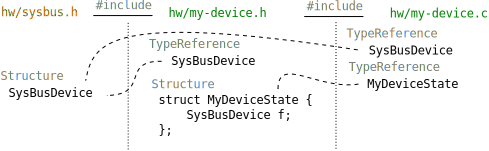
\includegraphics[height=0.31\textheight]{type-reference.png}
\end{center}

\vfill

Когда один тип в своём коде использует другой тип, то появляется
\textit{зависимость} между типами.
При зависимости от чужого типа, для её разрешения, генерируется включение
соответствующего заголовка, а при зависимости от своего типа
генерируется его код.
\end{frame}



\begin{frame}{Пример описания содержимого файла}
Устройство с одним регистром\\
\vfill
\begin{center}
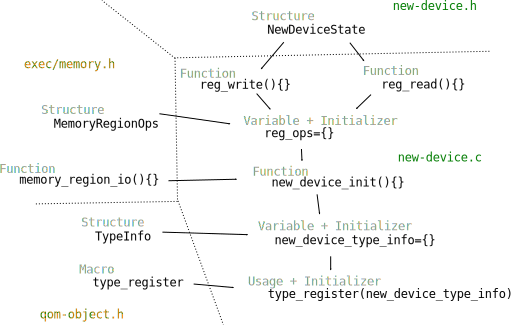
\includegraphics[height=0.75\textheight]{source-example.png}
\end{center}
\end{frame}



\begin{frame}{Пример вёрстки файла с исходным кодом}
\begin{minipage}{0.61\textwidth}
\includegraphics[width=1.15\linewidth]{c2600_pci_c_chunks.png}
\end{minipage}
\hfill
\begin{minipage}{0.34\textwidth}
\begin{itemize}
\item Топологическая сортировка
\item Семантическая сортировка
\item Оптимизация количества включаемых заголовков (транзитивное сокращение
графа включения)
\end{itemize}
\end{minipage}
\end{frame}



\begin{frame}{Анализ QEMU, взаимосвязь}
\begin{minipage}{0.35\textwidth}
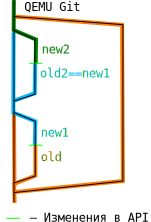
\includegraphics[height=0.8\textheight]{heuristics.png}
\end{minipage}
\hfill
\begin{minipage}{0.63\textwidth}
\begin{itemize}
\item Автоматический анализ заголовков QEMU
    \begin{itemize}
    \item Граф включения
    \item Макросы
    \end{itemize}
\item Эвристическая адаптация к изменениям API QEMU с привязкой к истории Git
\end{itemize}
\end{minipage}
\end{frame}



\section{Примеры применения инструмента}
\begin{frame}
\sectionpagekb
\begin{itemize}
\item PC на базе Intel Q35
\item Криптомаршрутизатор СISCO серии 2600 (C2621XM)
\end{itemize}
\end{frame}



\begin{frame}{PC на базе Intel Q35}
\begin{itemize}
\item Реализация Q35 уже имеется в QEMU и является одной из самых сложных.
\item Цель эксперимента~--- убедиться в эквивалентности предельных возможностей
предлагаемого метода (по сравнению с классическим, ручным).
\item Многие устройства в QEMU уже присутствовали.
\item Остальные были приведены в соответствие с действующими требованиями
QEMU при помощи инструмента.
\end{itemize}
\end{frame}



\begin{frame}{Схема Q35}
\begin{center}
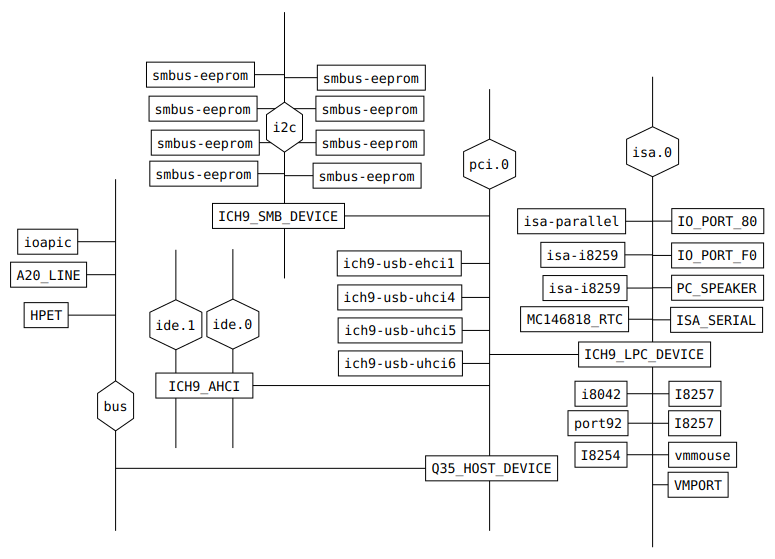
\includegraphics[width=\linewidth]{Q35-h.png}
\end{center}
\end{frame}



\begin{frame}{Статистика*}
\begin{center}
\begin{tabular}{l|lll}
Этап         & Затронуто & Вставлено & Удалено \\
             & файлов    & строк     & строк   \\
\hline
Подготовка** & 4         & 42        & 31      \\
Генерация    & 8         & 599       & 0       \\
Реализация   & 5         & 162       & 93***   \\
Суммарно     & 12        & 803       & 31      \\
\end{tabular}
\end{center}
\vfill
\it{*Статистика собрана с помощью git diff.}\\
\it{**Перенос необходимых символов в заголовочные файлы,
объявление глобальных переменных.}\\
\it{***Количество удаленных при реализации строк близко к количеству строк,
которые потребовалось исправить в сгенерированном коде.}
\end{frame}



\begin{frame}{Криптомаршрутизатор С2600 (C2621XM)}
\begin{itemize}
\item За основу взята реализация из Dynamips.
\item CPU PowerPC MPC860 изначально реализован без поддержки полносистемной
эмуляции.
\item Машина и все устройства (кроме CPU) были реализованы с помощью
инструмента.
\end{itemize}
\end{frame}



\begin{frame}{Схема C2621XM}
\begin{center}
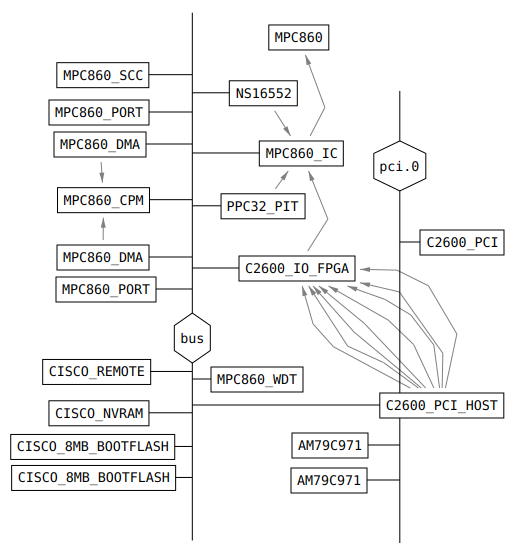
\includegraphics[height=0.8\textheight]{C2600.png}
\end{center}
\end{frame}



\begin{frame}{Статистика}
\begin{center}
\begin{tabular}{l|lll}
Этап         & Затронуто & Вставлено & Удалено \\
             & файлов    & строк     & строк   \\
\hline
Подготовка*  & 8         & 128       & 35      \\
Генерация    & 37        & 2186      & 0       \\
Реализация   & 31        & 4747      & 419     \\
Суммарно     & 45        & 6642      & 35      \\
\end{tabular}
\end{center}
\vfill
\it{*MMU, спец. регистры и прерывания CPU, идентификаторы PCI.}
\end{frame}



\begin{frame}{Статистика*}
\begin{center}
\begin{tabular}{l|ll}
Устройство        & Объём конфигурации & Сгенерировано \\
\hline
MPC860\_IC        & 6                  & 125           \\
C2600\_PCI\_HOST  & 6                  & 133           \\
C2600\_PCI        & 7                  & 82            \\
NS16552           & 7                  & 181           \\
C2600\_IO\_FPGA   & 8                  & 137           \\
CISCO\_REMOTE     & 7                  & 152           \\
AM79C971          & 12                 & 175           \\
\end{tabular}
\end{center}
\vfill
\it{*Объём кода приведён в строках.}
\end{frame}



\section{Заключение}
\begin{frame}
\sectionpagekb
\begin{itemize}
\item Результаты
\item Дальнейшая работа
\end{itemize}
\end{frame}



\begin{frame}{Результаты}
\begin{itemize}
\item Автоматизирован начальный этап разработки модели машины и устройства.
\item Настройка генерации осуществляется на языке Python.
\item Объём настройки генерации заготовки устройства в 11-25 раз меньше объёма
сгенерированной заготовки.
\item Разработан ГИП, включающий редактор машины, представленной в виде схемы.
\item Поддерживается разработка моделей машин, сравнимых по сложности с
Intel Q35.
\item Доля сгенерированного кода составляет от \(1/4\) до \(3/4\) в зависимости
от количества уже реализованных устройств.
\item Реализована взаимосвязь с существующим кодом QEMU, включая поддержку
разных версий API.
\end{itemize}
\end{frame}



\begin{frame}{Дальнейшая работа}
Отладочная обратная связь из запущенного эмулятора с информацией времени
выполнения.
\vfill
\begin{center}
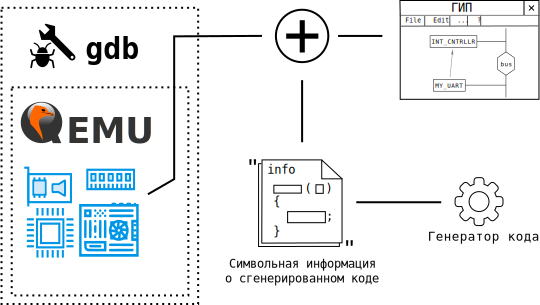
\includegraphics[width=0.8\textwidth]{gdb-feedback.png}
\end{center}
\end{frame}



\begin{frame}{Конец}
\begin{center}
Спасибо за внимание
\end{center}
\end{frame}



\end{document}
